% todo: fix figure using Jeffrey's powerpoint.
% decide on goal impact table for ``eye'' test. Make sure we are consistent in which season we are discussing (e.g. for Spezza).
% add discussion of Pettigrew, Kaplan, Diaz.
% penalties can be positive too (see action values).
% discuss rink bias (for things other than shot location).
% discuss other sports like soccer, basketball.
% Salary vs. Corsi, Fenwick.
%%%%%%%%%%%%%%%%%%%%%%% file typeinst.tex %%%%%%%%%%%%%%%%%%%%%%%%%
%
% This is the LaTeX source for the instructions to authors using
% the LaTeX document class 'llncs.cls' for contributions to
% the Lecture Notes in Computer Sciences series.
% http://www.springer.com/lncs       Springer Heidelberg 2006/05/04
%
% It may be used as a template for your own input - copy it
% to a new file with a new name and use it as the basis
% for your article.
%
% NB: the document class 'llncs' has its own and detailed documentation, see
% ftp://ftp.springer.de/data/pubftp/pub/tex/latex/llncs/latex2e/llncsdoc.pdf
%
%%%%%%%%%%%%%%%%%%%%%%%%%%%%%%%%%%%%%%%%%%%%%%%%%%%%%%%%%%%%%%%%%%%


\documentclass[runningheads,a4paper]{llncs}
\usepackage{amssymb}
\usepackage[T1]{fontenc}
\usepackage[font=small,labelfont=bf,tableposition=top]{caption}

\DeclareCaptionLabelFormat{andtable}{#1~#2  \&  \tablename~\thetable}
\setcounter{tocdepth}{3}
\usepackage{graphicx}

\usepackage{url}
\urldef{\mailsc}\path|{oschulte}@cs.sfu.ca|    
\newcommand{\keywords}[1]{\par\addvspace\baselineskip
	\noindent\keywordname\enspace\ignorespaces#1}

\def\set#1{\mathbf{#1}}
\newcommand{\mstate}{s}
\newcommand{\mfeatures}{\set{x}}
\newcommand{\impact}{\it{impact}}
\newcommand{\reward}{\it{R}}
\newcommand{\action}{a}
\newcommand{\actions}{A}
%\newcommand{\endmarker}{e}
\newcommand{\mstates}{S} % Markov states
\newcommand{\home}{H}
\newcommand{\away}{A}
\newcommand{\GD}{\it{GD}}
\newcommand{\MD}{\it{MD}}
\newcommand{\period}{\it{P}}
\newcommand{\zone}{\it{Z}}
\newcommand{\team}{T}
\newcommand{\neutral}{\it{Neutral}}
\newcommand{\history}{\it{h}}
%
%\graphicspath{{../}{../figures/}}
%this seems to be a list of directories
%\graphicspath{{../}}	
%%Example for automatically rescaling equations. 
% This is very tricky.
%\begin{equation}
%\label{eq:pimax}
%\resizebox{.55\textwidth}{!}{$
%\begin{split}
%P(\jtable_{2}|\set{E},\ttable) \propto &
%P(\keys = [jack,101],\it{Gr} = A, \it{Sat} = 1|\it{Int} = \class, \it{Rank} = 1, \it{Rat} = 3, \it{Diff}=1)\\
%\times & P(\keys = [jack,102],\it{Gr} = B, \it{Sat} = 2|\it{Int} = \class, \it{Rank} = 1, \it{Rat} = 2, \it{Diff}=2).
%\end{split}$
%}
%\end{equation}

%\usepackage{times}
%\usepackage[normaltitle,normalbib,normalmargins,normalindent]{savetrees}
%Example for automatically rescaling equations. 
% This is very tricky.
%\begin{equation}
%\label{eq:pimax}
%\resizebox{.55\textwidth}{!}{$
%\begin{split}
%P(\jtable_{2}|\set{E},\ttable) \propto &
%P(\keys = [jack,101],\it{Gr} = A, \it{Sat} = 1|\it{Int} = \class, \it{Rank} = 1, \it{Rat} = 3, \it{Diff}=1)\\
%\times & P(\keys = [jack,102],\it{Gr} = B, \it{Sat} = 2|\it{Int} = \class, \it{Rank} = 1, \it{Rat} = 2, \it{Diff}=2).
%\end{split}$
%}
%\end{equation}

%\usepackage{times}
%\usepackage[normaltitle,normalbib,normalmargins,normalindent]{savetrees}
\usepackage{amsmath}
\usepackage{amsfonts}
\usepackage{amssymb}
\usepackage{graphicx}
\usepackage{url}
%\usepackage{subfigure}
\usepackage{epstopdf}
\setcounter{MaxMatrixCols}{30}
%\usepackage{algorithm}
%\usepackage{algorithmic}
%\usepackage{subfigure}
%\usepackage{subcaption}
\usepackage{fancyhdr}
\usepackage{subfig}
\graphicspath{{../}{figures/}}

\DeclareMathOperator*{\argmax}{argmax}
\DeclareMathOperator*{\argmin}{argmin}
%\DeclareMathOperator{\pattern}{\pi}
\DeclareMathOperator{\Poly}{\mathbf{\mathrm{P}}}
\DeclareMathOperator{\RP}{\mathbf{\mathrm{RP}}}
%\DeclareMathOperator{\FP}{\mathbf{\mathrm{FP}}}
\DeclareMathOperator{\NP}{\mathbf{\mathrm{NP}}}
%\DeclareMathOperator{\E}{\mathbb{E}}
\renewcommand{\d}{\mathbf{d}}

\newcommand{\ZZ}{\mathbf{Z}}

\newcommand{\indep}{\ensuremath{\perp{}\!\!\!\!\!\!\!\perp{}}}
\newcommand{\dep}{\ensuremath{{\perp{}\!\!\!\!\!\!\!\not  \perp{}}}}
%\renewcommand{\L}{\mathcal{L}}
% variables denoting sets of nodes
\newcommand{\V}{V} 
\newcommand{\partC}{\mathcal{C}}
\newcommand{\pattern}{\pi}
% variables denoting nodes
\newcommand{\B}{B}
\renewcommand{\P}{P}
\newcommand{\R}{R}
\newcommand{\X}{X}
\newcommand{\Y}{Y}
\newcommand{\Z}{Z}
\newcommand{\F}{F}
\newcommand{\U}{U}
\newcommand{\W}{W}
\renewcommand{\S}{S}
\newcommand{\C}{C}
\newtheorem{mydef}{Proposition}
%variables for values
%\newcommand{\u}{u}
\renewcommand{\a}{a}
\renewcommand{\b}{b}
\newcommand{\z}{z}
\renewcommand{\v}{v}
\newcommand{\x}{x}
\newcommand{\y}{y}
\newcommand{\p}{p}
\newcommand{\s}{s}
\newcommand{\w}{w} % weights


%statistics
\newcommand{\divergence}{\it{D}}
\newcommand{\score}{\it{score}}
\newcommand{\confidence}{\it{conf}}
\newcommand{\support}{\it{support}}
\newcommand{\loglikelihood}{\it{LOG}}
\newcommand{\lof}{\it{LOF}}
\newcommand{\llmetric}{-L}
\newcommand{\lr}{\it{KLD}}
\newcommand{\kl}{\it{KL}}
\newcommand{\el}{\it{EL}}
\newcommand{\mi}{\it{MI}}
\renewcommand{\mid}{\it{ELD}}
\newcommand{\jid}{\it{JID}}
\newcommand{\roc}{\it{ROC}}
\newcommand{\outrank}{\it{OutRank}}
\newcommand{\knn}{\it{KNNOutlier}}
\newcommand{\auc}{\it{AUC}}
\newcommand{\eld}{\it{ELD}}
\newcommand{\fd}{\it{AD}}
\newcommand{\parameters}{\mathit{par}}
\newcommand{\bic}{\mathit{BIC}}
%random variables and graphical models
% number of values in the domain of a random variable
% variables for BNs
\newcommand{\domvals}{k}
\newcommand{\nodevalue}{\v}
\newcommand{\parvalue}{\mathbf{\pi}} % a single assignment of values to a set of 
%parents
\newcommand{\parvals}{l} % number of values of parent state.
\renewcommand{\r}{r} % CP-table row
\newcommand{\nbhd}{{\mathsf {nbdh}}}
\newcommand{\child}{\mathit{child}}
\newcommand{\parent}{\mathit{pa}}
\newcommand{\parents}{\mathbf{pa}}
\newcommand{\Parents}{\mathbf{PA}}
\newcommand{\family}{F} % families, family formulas
\newcommand{\vpi}{\mathbf{pa}} % for vectors of variable assignments
\renewcommand{\l}{\ell} % class label
\newcommand{\states}{r} % number of states of a variable
%\newcommand{\value}{value}
\newcommand{\mb}{\set{mb}} % markov blanket of a variable, vector-valued
\newcommand{\ssize}{N} % number of rows in join table; size of sample
\newcommand{\mbstates}{m} % number of states in Markov blanket
\newcommand{\frequency}{fr}
\newcommand{\pseudo}{\ast}
\newcommand{\counts}{+}
\newcommand{\weighted}{\ast}
\newcommand{\halpern}{H}
\newcommand{\instance}{I}

%logic notation
\newcommand{\iid}{iid~}
\newcommand{\predicate}{\phi}
\newcommand{\functor}{f}
\newcommand{\outdomain}{V}
\newcommand{\indomain}{\Omega}
\newcommand{\variable}{X} % first-order variable
\newcommand{\population}{\mathcal{P}}
\newcommand{\entity}{x}
\newcommand{\examplevar}{E}
\newcommand{\formula}{\f}
\newcommand{\formulas}{\mathcal{\phi}}
\newcommand{\literal}{l}
\newcommand{\conjunction}{\set{C}} % conjunction of literals
\newcommand{\fterm}{\f} % open function term
\newcommand{\fterms}{F} % set of function terms, also nodes in JBN
\newcommand{\term}{\sigma}
\newcommand{\Terms}{\bs{\sigma}}
\newcommand{\constant}{a}
\newcommand{\constants}{\bs{\constant}}
\newcommand{\gterm}{g} % ground term
\newcommand{\gterms}{\bs{\gterm}} %list of ground terms
\newcommand{\vterm}{x} % variable term
\newcommand{\vterms}{\bs{\vterm}} % list of variable terms
\newcommand{\assign}{A} % assignment of values to Bayes net
\newcommand{\resultset}{\mathbb{R}}
\newcommand{\grounds}{\#}
\newcommand{\grounding}{\gamma}
\newcommand{\groundall}{\Gamma}
\newcommand{\vars}{\mathit{Var}} % variables in a conjunction
\newcommand{\igraph}{I} % instance-level dependency graph.
\newcommand{\assignment}{\set{a}}
\newcommand{\atom}{\ell}
\newcommand{\gnode}{\alpha}
\newcommand{\gfamily}{\ground{f}}
\newcommand{\numformulas}{m}
\newcommand{\structure}{\mathcal{S}}
% logic programs
\newcommand{\program}{\mathcal{B}}
\newcommand{\clause}{\mathcal{c}}
\newcommand{\head}{\mathit{head}}
\newcommand{\body}{\mathit{body}}
\newcommand{\crule}{\mathit{cr}} % combining rule
\newcommand{\level}{\mathit{level}} % rank of function symbols in LP

%datbase schema
\newcommand{\rcolumns}{R}
\newcommand{\ecolumns}{E}
\newcommand{\dtable}{T} % can't use \table. Generic database table
\newcommand{\datatable}{D} % generic data table, not necessarily part of database.
\newcommand{\jtable}{J} % join table
\newcommand{\Ejoin}{$J^{+}$}
\newcommand{\jtables}{m}
\newcommand{\rtable}{R} % relationship table
\newcommand{\etable}{E} % entity table.
\newcommand{\ttable}{X} % target table
\newcommand{\nextended}{n}
\newcommand{\row}{r}
\newcommand{\rows}{\mathit{rows}}
\newcommand{\col}{j}
\newcommand{\cols}{\mathit{cols}}
\newcommand{\unary}{\f} % to denote a unary or attribute function
\newcommand{\numatts}{u} % to denote the number of unary or attribute functions.
\newcommand{\g}{g} % alternative for function
\newcommand{\relational}{\mathbf{r}} % denotes a generic relational functors, can be both relationship or descriptive attribute of relationship
\newcommand{\Relation}{R} % denotes a generic boolean relation
% a special type of literal conjunction that assigns a value %to each variable
\providecommand{\keywords}{\textbf{keywords: }}
\newcommand{\loss}{\ell}
\newcommand{\class}{c} % the class attribute
\newcommand{\classlabel}{y} % the class label
\newcommand{\classifier}{\mathcal{M}}
\newcommand{\target}{t} % target object
\newcommand{\Target}{T}
\newcommand*\rfrac[2]{{}^{#1}\!/_{#2}}
\newcommand{\object}{o}
\newcommand{\Class}{\mathcal{C}}
\newcommand{\Targetcount}{\Gamma}
\newcommand{\neighbor}{n}
\newcommand{\feature}{X} % feature or desc attribute of object or link
\newcommand{\features}{\bs{x}} % features 
\newcommand{\Features}{\bs{X}}
\newcommand{\ffunction}{\it{F}}
\newcommand{\attribute}{a} % nonclass attribute of target object
\newcommand{\attributes}{\bs{a}}
\newcommand{\rels}{\bs{R}} % chain of relationships.
\newcommand{\maxpath}{\rho}
\newcommand{\eatts}{\it{1Nodes}}
\newcommand{\ratts}{\it{2Nodes}}
\newcommand{\atts}{\it{ANodes}}
\newcommand{\marginalize}{\it{margin}}
%special functions
\newcommand{\AVG}{\it{AVG}}
\newcommand{\instances}{n} % counts number of occurrences in DB
\newcommand{\prob}{p} % frequency of formula true in in DB

%variables denoting graphs or models
\newcommand{\mln}{M}
\newcommand{\G}{G}
\newcommand{\node}{V}
\newcommand{\nodes}{V}
\newcommand{\edges}{E}
\newcommand{\clique}{C}
\newcommand{\cliques}{\mathcal{\clique}}
\newcommand{\cliquevalue}{c}
\newcommand{\graph}{G}
\newcommand{\M}{M}
\newcommand{\J}{J}
\renewcommand{\H}{H}
\newcommand{\K}{K} % component
\renewcommand{\O}{O} % oracle
%\renewcommand{\path}{\rho} % path, also foreignkey path
% Markov nets
\newcommand{\potential}{\Psi}
% database schema
\newcommand{\type}{\tau} % to denote a generic type
\newcommand{\E}{E} % for entity tables
\newcommand{\e}{e} % for specific entities
\newcommand{\f}{f}
\newcommand{\new}{\it{new}}
\renewcommand{\c}{c}
\renewcommand{\R}{R} % for relationship tables
\newcommand{\A}{A} % for attributes
\newcommand{\T}{T} % for tables generically
\newcommand{\New}{N}
\newcommand{\D}{\mathcal{D}} % for database instance
\newcommand{\databases}{\set{D}} % the number of databases
\newcommand{\vocab}{\mathcal{\L}} % for logical vocabulary associated with database
\newcommand{\name}{\mathit{name}} % generic attribute
\newcommand{\dom}{\mathit{dom}} % domain of attributes
\newcommand{\etables}{\alpha} % entity tables
\newcommand{\rtables}{\beta} % relationship table number
% specific constructs for examples


\newcommand{\team}{\it{T}}
\newcommand{\player}{\it{P}}
\newcommand{\match}{\it{M}}


\newcommand{\director}{\it{Director}}
\newcommand{\movie}{\it{Movie}}
\newcommand{\user}{\it{User}}
\newcommand{\corr}{\it{\rho}}
\newcommand{\student}{\mathit{Student}}
\newcommand{\I}{\mathit{I}}
\newcommand{\course}{\mathit{Course}}
\newcommand{\prof}{\mathit{Professor}}
\newcommand{\person}{\mathit{Person}}
\newcommand{\TA}{\mathit{TA}}
\newcommand{\actor}{\mathit{Actor}}
\newcommand{\age}{\mathit{age}}
\newcommand{\intelligence}{\mathit{intelligence}}
\newcommand{\diff}{\mathit{difficulty}}
\newcommand{\reg}{\mathit{Registered}}
\newcommand{\win}{\it{win}}
\newcommand{\ra}{\mathit{RA}}
\newcommand{\bt}{\mathit{blood type}}
\newcommand{\grade}{\mathit{grade}}
\newcommand{\gpa}{\mathit{gpa}}
\newcommand{\jack}{\mathit{Jack}}
\newcommand{\jill}{\mathit{Jill}}
\newcommand{\smith}{\mathit{Smith}}
\newcommand{\cmpt}{\mathit{CMPT120}}
\newcommand{\hi}{\mathit{Hi}}
% various constants
\newcommand{\true}{\mathit{T}}
\newcommand{\false}{\mathit{F}}
\newcommand{\normalconstant}{Z} % the normalization constant

% orderings
\newcommand{\pred}{\mathit{pred}}
%procedure names and such
\newcommand{\join}{\textsc{Join-Frequencies}}
\newcommand{\linus}{\textsc{Linus }}
\newcommand{\foil}{\textsc{Foil }}
\newcommand{\MLN}{\it{MLN}}
\newcommand{\MLNIDF}{\it{MLN-IDF}}
\newcommand{\tf}{\it{TF}}
\newcommand{\tfidf}{\it{TF-IDF}}
\newcommand{\Unigram}{\it{Unigram}}
\newcommand{\treetilde}{\textsc{TILDE }}



\begin{document}
	
	\mainmatter  % start of an individual contribution
	
	% first the title is needed
	\title{What is the Value of an Action in Ice Hockey? Learning a Q-function for the NHL}
	
	% a short form should be given in case it is too long for the running head
	\titlerunning{Learning a Q-function for the NHL}
	
	% the name(s) of the author(s) follow(s) next
	%
	% NB: Chinese authors should write their first names(s) in front of
	% their surnames. This ensures that the names appear correctly in
	% the running heads and the author index.
		\author{Oliver Schulte \and Zeyu Zhao \and Kurt Routley}
	%
	\authorrunning{Learning a Q-function for the NHL}
	% (feature abused for this document to repeat the title also on left hand pages)
	
	% the affiliations are given next; don't give your e-mail address
	% unless you accept that it will be published
	\institute{Simon Fraser University,\\
		Burnaby, BC, Canada\\
		\mailsc\\}
	
	%
	% NB: a more complex sample for affiliations and the mapping to the
	% corresponding authors can be found in the file "llncs.dem"
	% (search for the string "\mainmatter" where a contribution starts).
	% "llncs.dem" accompanies the document class "llncs.cls".
	%
	
	\toctitle{Lecture Notes in Computer Science}
	\tocauthor{Authors' Instructions}
	\maketitle
	
	
	\begin{abstract}
			Recent work has applied the Markov Game formalism from AI to model game dynamics for ice hockey, using a large state space. Dynamic programming is used to learn action-value functions that quantify the impact of actions on goal scoring. Learning is based on a massive dataset that contains over 2.8M events in the National Hockey League. As an application of the Markov model, we use the learned action values to measure the impact of player actions on goal scoring. Players are ranked according to the aggregate goal impact of their actions. We show that this ranking is consistent across across seasons, and compare it with previous player metrics, such as plus-minus and total points.
	\end{abstract}
	
%\keywords{Reinforcement Learning, Action-Value Functions, Player Rankings}
				
\section{Introduction}

This paper describes and extends a recent approach to sports analytics that applies advanced concepts from Artificial Intelligence to model game dynamics. This approach models game dynamics using Markov games~\cite{Littman1994}, a multi-agent extension of Markov Decision Processes. A Markov game model can answer a fundamental question about a sport: Which actions contribute to winning in what situation? 

We approach this question for ice hockey by learning an {\em action-value function}, or Q-function, for a Markov game model of the National Hockey League (NHL). In reinforcement learning (RL) notation, the expression $Q(\mstate,\action)$ denotes the expected reward of taking action $\action$ in state $\mstate$.
 We learn a Q-function from a massive dataset about matches in the National  Hockey League (NHL). This dataset comprises all play-by-play events from 2007 to 2014, for a total of over 2.8M events/actions and almost 600K play sequences.
%after 2007, the format was standardized on nhl.com, and they had complete data about which players were on the ice.
The Markov Game model comprises over 1.3M states. Whereas most previous works on Markov Game models aim to compute optimal strategies or policies \cite{Littman1994}, 
%(i.e., minimax or equilibrium strategies), 
we learn a model of how hockey is actually played, and do not aim to compute optimal strategies. In RL terminology, we learn a Q-function for  the {\em on-policy} setting \cite{bib:sutton}. 
%In RL notation, the expression $Q(\mstate,\action)$ denotes the expected reward of taking action $\action$ in state $\mstate$.
%
%\paragraph{Motivation.}
Motivation for learning a Q-function for NHL hockey dynamics includes knowledge discovery and player evaluation, which is the application we focus on in this paper.

{\em Knowledge Discovery.} The Markov Game model provides information about the likely consequences of actions. The basic model and algorithms can easily be adapted to study different outcomes of interest, such as goals and penalties.
For example, with goals as rewards, a Q-function specifies the impact of an action on future goals. With penalties as costs in the same model, the resulting Q-function specifies the impact of an action on future penalties. 

%In a finalist paper at the MIT Sloan conference, Cervone {\em et al.} learned a Q-function for basketball. They asserted that ``most questions that coaches, players, and fans have about basketball, particularly those that involve the offense, can be phrased and answered in terms of EPV [i.e. the Q-function].''

{\em Player Evaluation.} One of the main tasks for sports statistics is evaluating the performance of players \cite{Schumaker2010}.
A common approach is to assign action values, and sum the corresponding values each time a player takes the respective action.
%An advantage of this additive approach is that it provides highly interpretable player rankings. 
A simple and widely used example in ice hockey is the +/- score: for each goal scored by (against) a player's team when he is on the ice, add +1 (-1) point. 
Researchers have developed several extensions of +/- for hockey \cite{Macdonald2011a,Spagnola2013,Schuckers2013}. The NHL has started publishing advanced player statistics such as the Corsi (Shot Attempts) and Fenwick (Unblocked Shot Attempts) ratings.\footnote{\url{nhl.com}}
Using action values defined by the Q-function has two major advantages compared to 
the previous action count approaches used in ice hockey. (1) The Markov game model is aware of the {\em context} of actions within a game. In the Markov Game model, \emph{context  = state.} 
%For example, a goal is more valuable in a tied-game situation than when the scorer's team is already four goals ahead \cite{Pettigrew2015}. 
%Another example is that if a team manages two successive shots on goal, the second attempt typically has a higher chance of success. 
%Formally, the Q function depends {\em both} on the state $\mstate$ and the action $\action$. 
%Richer state spaces therefore capture more of the context of an action. 
(2) An action may have medium-term and/or ripple effects rather than immediate consequences. For example, penalties have a short-term but not immediate effect on goal scoring.
 %in terms of visible rewards like goals. 
Therefore evaluating the impact of an action requires {\em look-ahead}, which the Q-function provides.  
%Long-term lookahead is especially important in ice hockey because evident rewards like goals occur infrequently \cite{Lock2009}.
%For example, if a player receives a penalty, this leads to a manpower disadvantage for his team, known as a powerplay for the other team.
%It is easier to score a goal during a powerplay, but this does not mean that a goal will be scored immediately after the penalty. 
%For another example, if a team loses the puck in their offensive zone, the resulting counterattack by the other team may lead to a goal eventually but not immediately. 
%The dynamic programming value iteration algorithm of Markov Decision Processes provides a computationally efficient way to perform unbounded lookahead.

%\paragraph{Evaluation} Our evaluation learns Q-functions for two reward events, scoring the next goal and receiving the next penalty. We observe a wide variance of the impact of actions with respect to states, showing context makes a substantial difference. We provide examples of the context dependence to give a qualitative sense of how the Markov Game model accounts for context. %To evaluate the impact of propagating action effects, we provide evidence that including state transitions across play sequences reduces the uncertainty (entropy) about which team scores the next goal.
To evaluate player performance, we use the Q-function to quantify the value of a player's action in a context. The action values are then aggregated over games and seasons to get player impact scores. Player impact scores correlate with plausible alternative scores, such as a player's total points, but improve on these measures, as our impact score is based on many more events. A new finding is that player impact on goals correlates well across seasons ($r = 0.7$).

\paragraph{Contributions.}
We make our extensive dataset available on-line, in addition to our code and the learned Markov game model \cite{bib:sports-site}.
The main contributions of this paper may be summarized as follows:

\begin{enumerate}
\item We describe a set of recent developments that apply Markov game modelling to sports analytics. Learning a Q-function provides context-aware action values to score hockey player actions based on look-ahead from the current game context.
\item We show that the resulting player rankings are consistent across seasons.
%\item The first application of reinforcement learning in a continuous-flow sports domain,
%\item A new and intuitive method for analyzing player actions within the context of a game.
\end{enumerate}

%\paragraph{Paper Organization.}
%
%We review related work in measuring player contributions and machine learning in sports in Section~\ref{sec:related-work}. We then give some background information on the ice hockey domain and NHL play-by-play sequences data. Our Markov Game model translates the hockey domain features into the Markov formalism. We describe how we implement a scalable value iteration for the ice hockey domain. The evaluation section addresses the impact of context and lookahead.
%%, the two main advantages of the Markov model.
%We apply the model to rank the aggregate performance of players and describe the resulting player ranking. We view our work as taking the first step, not the last, in applying AI modelling techniques to ice hockey.
%Therefore, we conclude with a number of potential extensions and open problems for future work.

\section{Related Work} This paper is an extension of our previous work~\cite{Routley2015a}. The closest predecessor to our work in ice hockey is the Total Hockey Rating (THoR) \cite{Schuckers2013}. This assigns a value to all actions, not only goals. Actions were evaluated based on whether or not a goal occurred in the following $20$ seconds after an action. %For penalties, the duration of the penalty was used as the lookahead window.
This work used data from the $2006/2007$ NHL season only. THoR assumes a fixed value for every action and does not account for the context in which an action takes place. Furthermore, the window of $20$ seconds restricts the look-ahead value of each action. %Our Q-learning method is not restricted to any particular time window for lookahead.

The Win-Probability-Added player metric \cite{Pettigrew2015,Kaplan2014} scores the importance of a goal relative to the game context. This work uses a Markov model as well, which is a submodel of ours in the following sense: (1) The only actions considered are goals. (2) The context includes the current goal and manpower differentials, but not the period and not the recent play history. Their work does, however, include the current game time, unlike our model. The game time is especially important for propagating the impact of an action to a final win, since for instance the probability of a win is 1 if a goal puts a team ahead in the last minute.

In a finalist paper at the MIT Sloan conference, \cite{Cervone2014a} Cervone {\em et al.} used spatial-temporal tracking data for basketball to build the {\sc Pointwise} model for valuing player decisions and player actions. Conceptually, their approach to defining action values is the closest predecessor to ours: The counterpart to the value of a state in a Markov game is called expected possession value (EPV). The counterpart to the impact of an action on this value is called EPV-added (EPVA). Cervone {\em et al.} emphasize the potential of the context-based impact definitions for knowledge discovery: ``we assert that most questions that coaches, players, and fans have about basketball, particularly those that involve the offense, can be phrased and answered in terms of EPV [i.e., the Q-function].'' While the definition of action impact is conceptually very similar, \cite{Cervone2014a} use neither AI terminology nor AI techniques. Moreover, the NHL does not yet have and therefore we do not use spatial tracking data, which is the main focus of \cite{Cervone2014a}. 

Cervone {\em et al.}~\cite{Cervone2014} note that the Q-function approach for valuing actions can in principle be applied to different types of sports. 
Substantially smaller Markov Decision Process Models than ours have been used to model dynamics in various sports; for a review please see \cite{Cervone2014a} and \cite{Routley2015a}. To our knowledge these models have not been applied to valuing actions. 




\section{Hockey Data Used}
\label{sec:background-notation}

We assume familiarity with the basic rules of NHL play%~\cite{NHL2014}
; \cite{Routley2015a} provides a brief summary.
%
%We outline the rules of hockey and describe the dataset available from the NHL.
%
%\subsubsection{Hockey Rules.}
%%We describe a Markov Game Model for ice hockey. To motivate our model, we
%%We give a brief overview of rules of play in the NHL~\cite{NHL2014}. 
%NHL games consist of three periods, each 20 minutes in duration. A team has to score more goals than their opponent within three periods in order to win the game. If the game is still tied after three periods, the teams will enter a fourth overtime period, where the first team to score a goal wins the game. If the game is still tied after overtime during the regular season, a shootout will commence. During the playoffs, overtime periods are repeated until a team scores a goal to win the game. Teams have five skaters and one goalie on the ice during even strength situations.
%Penalties result in a player sitting in the penalty box for two, four, or five minutes and the penalized team will be shorthanded, creating a manpower differential between the two teams.
%The period where one team is penalized is called a powerplay for the opposing team with a manpower advantage.
%A shorthanded goal is a goal scored by the penalized team, and a powerplay goal is a goal scored by the team on the powerplay.
The NHL provides information about sequences of play-by-play events, which are scraped from \url{http://www.nhl.com} and stored in a relational database. The real-world dataset is formed from $2,827,467$ play-by-play events recorded by the NHL for the complete 2007-2014 seasons, regular season and playoff games, and the first 512 games of the 2014-2015 regular season. A breakdown of this dataset is shown in Table~\ref{table:size-of-dataset} (left).
%Table~\ref{table:size-of-dataset}. %Note that there are only 30 teams in the NHL, but some teams were replaced and moved to new locations, so there are 32 teams in our dataset.
%For each event, the current goal differential $GD$, manpower differential $MD$, and period $P$ are scraped from the play-by-play data.
The type of events recorded by the NHL from the 2007-2008 regular season and onwards are listed in Table~\ref{table:size-of-dataset}. There are two types of events: actions performed by players and start and end markers for each play sequence. Every event is marked with a continuous time stamp, and every action is also marked with a zone $Z$ and which team, Home or Away, carries out the action.


\begin{table}[htb]
\caption{Left: Size of Dataset. Right: NHL Play-By-Play Events Recorded}
\label{table:size-of-dataset}
\begin{center}
\begin{tabular}{|l|c|}
\hline
\bf{Number of Teams} & 32 \\ \hline
\bf{Number of Players} & 1,951 \\ \hline
\bf{Number of Games} & 9,220 \\ \hline
\bf{Number of Sequences} & 590,924 \\ \hline
\bf{Number of Events} & 2,827,467 \\ \hline
\end{tabular}
\quad
\begin{tabular}{|l|l|}
\hline
 \bf{Action Event} & \bf{Start/End Event}\\ \hline
Face-off & Period Start \\\hline
Shot & Period End \\\hline
Missed Shot & Early Intermission Start\\ \hline
Blocked Shot & Penalty\\ \hline
Takeaway & Stoppage\\  \hline
Giveaway & Shootout Completed\\ \hline
Hit & Game End\\ \hline
Goal & Game Off\\ \hline
& Early Intermission End \\
\hline
\end{tabular}
\end{center}
\end{table}

%\begin{table}[htb]
%\caption{NHL Play-By-Play Events Recorded}
%\label{table:events-recorded}
%\begin{center}
%\begin{tabular}{|l|l|}
%\hline
% \bf{Action Event} & \bf{Start/End Event}\\ \hline
%Faceoff & Period Start \\\hline
%Shot & Period End \\\hline
%Missed Shot & Early Intermission Start\\ \hline
%Blocked Shot & Penalty\\ \hline
%Takeaway & Stoppage\\  \hline
%Giveaway & Shootout Completed\\ \hline
%Hit & Game End\\ \hline
%Goal & Game Off\\ \hline
%& Early Intermission End \\
%\hline
%\end{tabular}
%\end{center}
%\end{table}


\section{Markov Games}
A Markov Game \cite{Littman1994}, is defined by a set of states, $\mstates$, and a collection of action sets, one for each agent in the environment. State transitions are controlled by the current state and one action from each agent. A state transition is associated with a reward for each agent. In our hockey Markov game model, there are two players, the Home Team $\home$ and the Away Team $\away$.
%
In each state, only one team performs an action, although not in a turn-based sequence.
This reflects the way the NHL records actions.
%Thus at each state of the Markov Game, exactly one player chooses No-operation.
%State transitions follow a semi-episodic model \cite{bib:sutton} where play moves from episode to episode, and information from past episodes is recorded as a list of {\em context features}. The past information includes the goal score and manpower. 
 %{\em Within} each episode/sequence, our game model corresponds to a game tree with perfect information as used in AI game research \cite{Russell2010}. 
%

%\subsection{State Space}
%We begin by defining the Markov game state space. 
A \textbf{state} comprises context features and play sequences that represent the recent trajectory of the game. A sequence in the NHL play-by-play data corresponds to an episode in Markov decision process terminology.
% add reference to basketball. We define context features, then play sequences.

%\begin{table}[htdp]
%\caption{Context Features}
%\label{table:context-features}
%\begin{center}
%%\resizebox{1\columnwidth}{!}{
%%\begin{tabular}{|c|c|p{2cm}|c|}
%\begin{tabular}{|c|c|c|}
%\hline
%Notation & Name & Range \\\hline
%$\GD$ & Goal Differential & [-8,8]\\ \hline
%$\MD$ & Manpower Differential & [-3,3]\\ \hline
%$\period$ & Period & [1,7]\\\hline
%\end{tabular}
%}
%\end{center}
%\label{default}
%\end{table}%


\paragraph{Context Features} remain constant throughout a play sequence (episode). 
%Previous work on Markov process models for ice hockey 
%%\cite{Thomas2013} 
%defined states in terms of hand-selected features that 
%Relevant features for hockey include the current goal and manpower differentials and penalties.
%We refer to such features as \textbf{context features}. Context features remain the same throughout each play sequence.
%
A \textbf{context state} lists the values of relevant features at a point in the game. 
These features are shown in Table~\ref{table:play-by-play-data}(left), together with the range of integer values observed. Goal Differential $GD$ is calculated as Number of Home Goals - Number of Away Goals. A positive (negative) goal differential means the home team is leading (trailing).  Manpower Differential $MD$ is calculated similarly.
%as Number of Home Skaters on Ice - Number of Away Skaters on Ice. A positive manpower differential typically means the home team is on the powerplay (away team is penalized), and a negative manpower differential typically means the home team is shorthanded (away team is on the powerplay). 
Period $P$ represents the current period number the play sequence occurs in, typically ranging in value from 1 to 5. Periods 1 to 3 are the regular play of an ice hockey game, and periods 4/5 indicate overtime/shootout periods.

\begin{table}[htb]
\caption{The Markov Game State Space. Left: Context Features. Right: Play Sequences in Tabular Format. A \textbf{play sequence} $\history$ is a sequence of events starting with exactly one start marker, followed by a list of action events, and ended by at most one end marker.  Start and end markers are shown in Table~\ref{table:size-of-dataset}(Right), adding shots and face-offs as start markers, and goals as end markers. }
\label{table:play-by-play-data}
\begin{center}
\resizebox{0.25\columnwidth}{!}{
\begin{tabular}{|c|c|}
\hline
 Name & Range \\\hline
 Goal Diff. & [-8,8]\\ \hline
 Manpower Diff.& [-3,3]\\ \hline
 Period & [1,7]\\\hline
\end{tabular}
}
\resizebox{0.7\columnwidth}{!}{
\quad
\begin{tabular}{|l|l|l|l|c|}
\hline
\bf{GameId} & \bf{Period} & \bf{Sequence \# } & \bf{Event \#} & \bf{Event} \\ \hline
1 & 1 & 1 & 1 & PERIOD START \\ \hline
1 & 1 & 1 & 2 &  (Home,Neutral) \\ \hline
1 & 1 & 1 & 3 & hit(Away,Neutral) \\ \hline
1 & 1 & 1 & 4 & takeaway(Home,Defensive) \\ \hline
1 & 1 & 1 & 5 & missed\_shot(Away,Offensive) \\ \hline
1 & 1 & 1 & 6 & shot(Away,Offensive) \\ \hline
1 & 1 & 1 & 7 & giveaway(Away,Defensive) \\ \hline
1 & 1 & 1 & 8 & takeaway(Home,Offensive) \\ \hline
1 & 1 & 1 & 9 & missed\_shot(Away,Offensive) \\ \hline
1 & 1 & 1 & 10 & goal(Home,Offensive) \\ \hline
1 & 1 & 2 & 11 & face-off(Away,Neutral) \\ \hline
\multicolumn{5}{|c|}{\ldots} \\ \hline
\end{tabular}
}
\end{center}
\end{table}


%\begin{description}
%\item[Goal Differential $GD$] is calculated as Number of Home Goals - Number of Away Goals. A positive (negative) goal differential means the home team is leading (trailing).
%\item[Manpower Differential $MD$] is calculated as Number of Home Skaters on Ice - Number of Away Skaters on Ice. A positive manpower differential typically means the home team is on the powerplay (away team is penalized), and a negative manpower differential typically means the home team is shorthanded (away team is on the powerplay).
%\item[Period $P$] represents the current period number the play sequence occurs in, typically ranging in value from 1 to 5. Periods 1 to 3 are the regular play of an ice hockey game, and periods 4 and onwards are for overtime and shootout periods.
%\end{description}

%  Manpower Differential $MD$ 
%  \footnote{Pulling the goalie can also result in a skater manpower advantage.} 
%  Period $P$ represents the current period number the play sequence occurs in, typically ranging in value from 1 to 5. Periods 1 to 3 are the regular play of an ice hockey game, and periods 4 and onwards are for overtime and shootout periods as needed.
%%
%Potentially, there are $(17 \times 7 \times 7) = 833$ context states. In our NHL dataset, $450$  context states occur at least once.

\paragraph{Play Sequences} are sequences of actions.
\label{subsec:play-sequences}
%[recent trajectory from baseball paper]
%Previous research on Markov process models of hockey has used only context features such as those described in Section~\ref{sec:context}. A Markov process model can answer questions such as how goal scoring or penalty rates depend on the game context \cite{Thomas2013}. However, in this paper our focus is on the impact of a player's actions on a game.
The basic action events are shown in Table~\ref{table:play-by-play-data}. 
%These represent the recent trajectory of a match. The basic set of 8 possible actions is listed in Table~\ref{table:size-of-dataset} (Right). %\ref{table:events-recorded}. 
Each of these actions has two parameters: which team $T$ performs the action and the zone $\zone$ where the action takes place. Zone $Z$ represents the area of the ice rink in which an action takes place, relative to the team performing an action
(Offensive, Neutral, Defensive). 
%An \textbf{action sequence} or \textbf{play sequence} is a sequence of actions. 
Table~\ref{table:play-by-play-data} shows an example of a NHL play-by-play action sequence in tabular form. %For example, $Z = $ Offensive zone relative to the home team is equivalent to $Z = $ Defensive zone relative to the away team. 
%A specification of an action plus parameters is an \textbf{action event}. 
%Using action description language notation \cite{bib:LevesquePirriReiter98}, we write action events in the form $\action(\team,\zone)$. 
%
%For example, $\it{faceoff}(\it{Home},\neutral)$ denotes the home team wins a faceoff in the neutral zone. We usually omit the action parameters from generic notation and write $\action$ for a generic action event.
%
%We also allow empty history $\emptyset$ as a valid play sequence. 
%A \textbf{complete} play sequence ends with an end marker.
A \textbf{state} is a pair $\mstate = \langle \mfeatures, \history \rangle$ where $\mfeatures$ is a list of context features and $\history$ a play/action sequence. %State $\mstate$ represents a play sequence consisting of action events $a_1,a_2,\ldots,a_n$ and with a particular $GD$, $MD$, and $P$ as the context. If the sequence $\history$ is empty, then state $s$ is purely a context node. 
%Potentially, there are $(7 \times 2 \times 3)^{40} = 42^{40}$ action histories. In our dataset, 1,325,809 states, that is, combinations of context features and action histories, occur at least once. 


\paragraph{State Transitions.}
\label{subsec:transitions}

If $\history$ is an incomplete play sequence, we write $\history \star \action$ for the play sequence that results from appending $\action$ to $\history$, where $\action$ is an action event or an end marker.
Similarly if $\mstate = \langle \mfeatures, \history \rangle$, then $\mstate \star \action \equiv \langle \mfeatures, \history \star \action \rangle$ denotes the unique successor state that results from executing action $\action$ in  $\mstate$.
%This notation utilizes the fact that context features do not change until an end marker is reached.
%For example, the goal differential does not change unless a goal event occurs.
%If $\history$ is a complete play sequence, then the state $\langle \mfeatures, \history \rangle$ has a unique successor $\langle \mfeatures', \emptyset \rangle$, where the mapping from $\mfeatures$ to $\mfeatures'$ is determined by the end marker.
%For instance, if the end marker is $\it{goal}(Home,*)$, then the goal differential increases by 1.
State transition examples are shown in Figure~\ref{fig:state-transition-graph}. Since the complete action history is encoded in the state, action-state pairs are equivalent to state pairs.
%Therefore we can model transitions from state to state only, rather than transitions from state to state given an action, even though we are mainly interested in the effects of actions.
%For example, we can write $Q(\mstate \star \action)$ to denote the expected reward from taking action $\action$ in state $\mstate$, where $Q$ maps states to real numbers, rather than mapping action-state pairs to real numbers, as is more usual.
%Note that $R(s)$ is the reward value for the state, and will be discussed in Section~\ref{subsec:reward}.
%In Figure~\ref{fig:state-transition-graph}, the reward encodes the objective of scoring a goal.

%\begin{figure}[htbp]
%\includegraphics[width = 0.5\columnwidth]
%{transition}
%\quad
%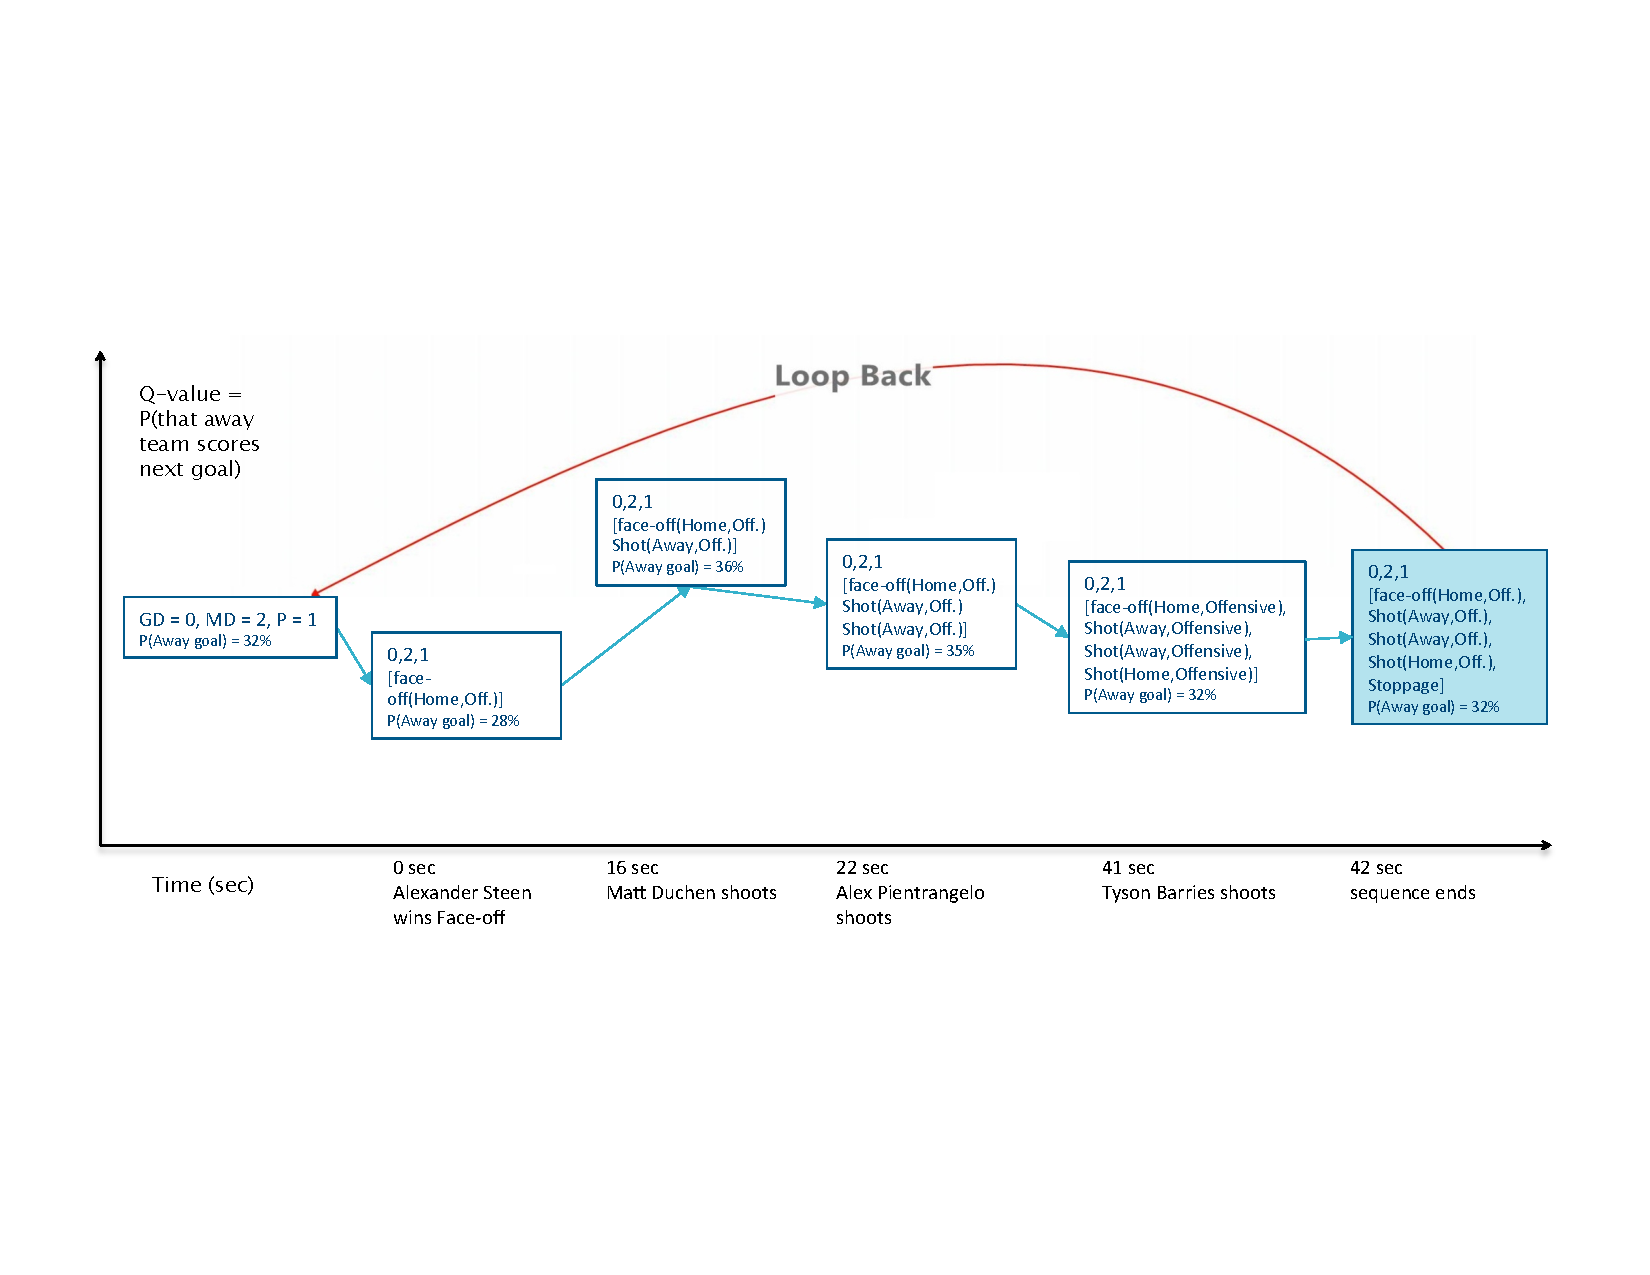
\includegraphics[width = 0.9\columnwidth]{q-ticker}
%\caption{Top: State Transition Examples. We omit some positive probability transitions for simplicity. After an action occurs, it is recorded as part of the next state. Bottom: The Q-Value Ticker tracks the change in state value during a game. In this example, Colorado (Home) plays St. Louis (Away), 1st period, 8th play sequence. The Q-value represents the probability that St. Louis scores the next goal.}
%\label{fig:state-transition-graph}
%\end{figure}

\begin{figure}[htbp]
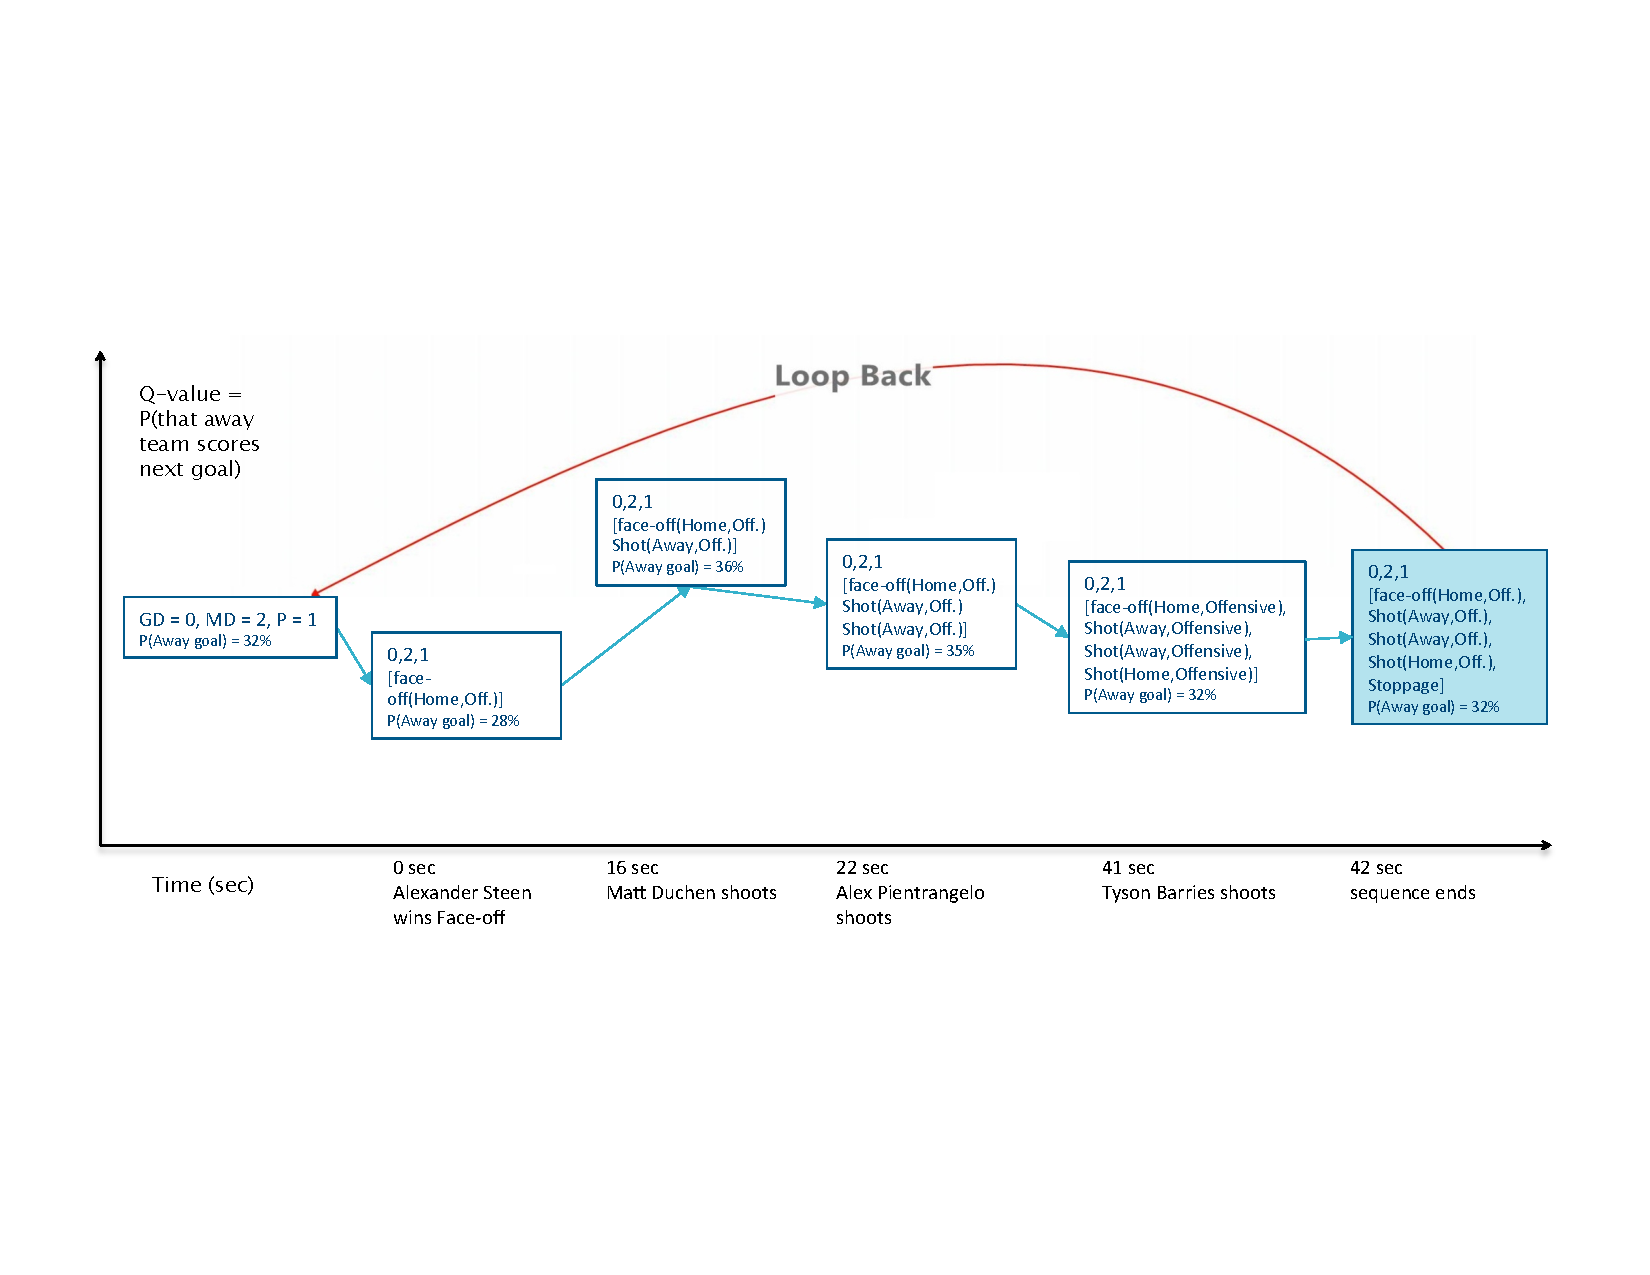
\includegraphics[width = 1\columnwidth]{q-ticker}
\caption{The Q-Value Ticker tracks the change in state value during a game. In this example, Colorado (Home) plays St. Louis (Away), 1st period, 8th play sequence. The Q-value represents the probability that St. Louis scores the next goal.}
\label{fig:state-transition-graph}
\end{figure}


\paragraph{Rewards and the Q-Function.} Important reward/cost events for hockey include goals, penalties \cite{Routley2015a}, and final wins~\cite{Routley2015}.
This paper examines goal scoring, represented by the following reward function. Any state ending with a home (away) goal is an absorbing state, where the home (away) team receives a reward of 1. For other states the reward is 0. 
%
%
%\begin{enumerate}
%\item For any state $\mstate$ with a complete play sequence that ends in a Home resp. Away goal, we set $\reward_{\home}(\mstate) := 1$ resp. $\reward_{\away}(\mstate) := 1$. For other states the reward is 0.
%\item Any state $\mstate$ with a complete play sequence that ends in a Home resp. Away goal is an absorbing state (no transitions from this state).
%\end{enumerate}
%
%A strength of Markov Game modelling is that the same model and computations (e.g., value iteration) can be applied to many reward functions depending on what results are of interest. 
% estimates the impact of events with regard to the final score.
%
%The action-value function $Q(\mstate\star\action)$ represents the expected reward given that action $\action$ is taken in state $\mstate$
%\cite{bib:sutton}. 
With this Next Goal reward function, the expected reward $Q_{\home}(\mstate)$
%
represents the probability that if play starts in state $\mstate$, a random walk through the state space of unbounded length ends with a goal for the Home team resp. the Away team. Given the transition probabilities in the Markov game model, the Q-function values can be computed by dynamic programming  \cite{Routley2015a}.
%using a Bellman equation
%$$Q_{i+1}(s) := R(s) + \frac{1}{Occ(s)}\sum_{(s,s') \in E}(Occ(s,s')\times Q_{i}(s')).$$


\section{Action Values and Player Impact Rankings.}
%We discuss the results of action values in Section~\ref{subsec:action-values} and player values in Section~\ref{subsec:player-valuations}.
%\subsection{ACTION IMPACT VALUES}
\label{subsec:action-values}


The \textbf{impact} of an action is a function of context (= Markov state), defined as follows:

\begin{equation}
\impact(\mstate,\action) \equiv Q_{\team}(\mstate \star \action) - Q_{\team}(\mstate)
\end{equation}

where $\team$ is the team executing the action $\action$. 
%
%In a zero-sum game, the state value is usually defined as the final result following optimal play \cite{Russell2010}. Intuitively, the value specifies which player has a better position in a state. Since we are not modelling optimal play, but actual play in an on-policy setting, the expected difference in rewards is the natural counterpart. 
%
The impact quantity measures how performing an action in a state affects the expected reward difference. Figure~\ref{fig:state-transition-graph} shows a ``Q-value ticker'' representation of how the Q-values for the Next Goal reward change with state transitions in a specific game sequence \cite{Cervone2014a}. The impact measures the magnitude of the Q-value change when an action takes the match from one state to another. This change measures the impact of an action on the {\em chance} of scoring the next goal. The Next Goal Q-values  are very different from simply counting goals, in at least two respects. (1) {\em The Next Goal Q-values reflect both offensive and defensive contributions.} For example, if a player wins a face-off in his defensive zone, this decreases the chance that the opposing team will score the next goal, and therefore increases the chance that his team will score the next goal.  
(2) The look-ahead of the Q-value computation means that {\em actions that lead to goals, not only goals themselves, receive high impact counts.} Routley and Schulte report that averaged over states, shots have the highest goal impact compared to other actions \cite{Routley2015a}, as one would expect. They show that {\em depending on the context and event history, the value of an action can vary greatly.} All actions, including penalties, but excluding goals and face-offs won in the offensive zone, have at least one conext (state) where the action has a positive impact, and another context with a negative impact.


%\begin{figure}[htbp]
%\includegraphics[width = 0.9\columnwidth]
%{q-ticker}
%%\vspace{1in}
%\caption{Q-value Ticker. Colorado (Home) plays St. Louis (Away), 1st period, 8th play sequence. The Q-value represents the probability that St. Louis scores the next goal.}
%\label{fig:q-ticker}
%\end{figure}
%
%Figure~\ref{fig:boxplot-action-values} shows a boxplot for the action impact values as they range over different contexts, i.e., states in the Markov Game model.
%
%(Boxplots produced with MATLAB R2014a.)
%The red dots are outliers beyond 2.7 s.d.
%A cutoff of -0.2 and 0.2, shown by the horizontal dashed line, was used for the impact values on both boxplots. While the Q-values are based on the frequency of states, we weight all states equally in discussing the properties of the Q-function. The boxplot does not include Q-values for states whose frequency is below 5\%.
%
%\subsection{Action Impact Values Depend on Context}

%The context-dependence is observed for both scoring goals and receiving penalties.
%
%\paragraph{Impact on Scoring the Next Goal.} 
%\footnote{Assuming the frequency of the state is at least 5\%}. 
%Two examples of how the value of the same action can depend on the context include the following, which we found by examining states with extreme impact values.
%
%{\em Blocked Shot.} Blocking the first shot on net when killing a penalty decreases a team's scoring rate $(impact=-0.0864)$. But blocking the second shot on net increases the scoring rate $(impact=0.1399)$.
%
%{\em Penalty.} Receiving a penalty when on the powerplay is very bad $(impact=-0.1789)$. But if a player, while on the penalty kill, receives a penalty while goading their opponent into an offsetting penalty, the penalty actually increases their team's scoring rate $(impact=0.0474)$.
%
%The THoR player ratings compute the impact of actions based on goals that immediately follow the action (\cite{Lock2009,Schuckers2011}; see Section~\ref{sec:related-work}).
%%The values given for each action in \cite{Lock2009} are displayed as an asterisk in Figure~\ref{fig:goal-impact}.
%%
%The THoR values
%%\cite{Lock2009}
%agree with our median goal impact values in terms of whether an action generally has positive or negative impact. For example, penalties are known to generally be good for the opposing team, and shots are good for the shooter's team. THoR values are close to the median Markov model impact values for 6 out of 10 action.%
%This comparison suggests THoR aggregates action values over many contexts the Markov game models explicitly. A lesion study provides further support for this comparison.
% described in the supplementary material, we examine directly defining the value of an action as the average impact of the action over all states. Using the averge impact as a fixed action value leads to a loss of information, as measured by the entropy of the prediction for which team scores the next goal. 
% Another lesion study assesses the importance of propagating information between states, especially from one play sequence to subsequent ones. The results show that goal impact values of the actions change substantially depending on how much information the model propagates.

\subsection{Single Season Player Valuations.}
\label{subsec:player-valuations}


\begin{table}[htb]
\caption{2014-2015 Top-25 Player Impact Scores For Goals}
\label{table:top-player-impact-goals}
\begin{center}
\resizebox{1\textwidth}{!}{
\begin{tabular}{|l|c|c|c|c|c|c|r|}
\hline
\bf{Name} & \bf{Position} & \bf{Goal Impact} & \bf{Goals} & \bf{Points} & \bf{+/-} & \bf{Takeaways} & \bf{Salary} \\ \hline
Jori Lehtera & C & 17.29 & 8 & 25 & 13 & 21 & \$3,250,000 \\ \hline
Henrik Zetterberg & LW & 14.54 & 7 & 30 & -1 & 21 & \$7,500,000 \\ \hline
Jason Spezza & C & 14.33 & 6 & 25 & -11 & 25 & \$4,000,000 \\ \hline
Vladimir Tarasenko & RW & 12.78 & 20 & 37 & 18 & 20 & \$900,000 \\ \hline
Jonathan Toews & C & 12.60 & 13 & 29 & 9 & 19 & \$6,500,000 \\ \hline
Joe Pavelski & C & 12.22 & 16 & 29 & 5 & 22 & \$6,000,000 \\ \hline
Kyle Okposo & RW & 11.79 & 8 & 29 & -4 & 18 & \$3,500,000 \\ \hline
Brent Burns & D & 11.56 & 10 & 27 & -3 & 16 & \$5,760,000 \\ \hline
Gustav Nyquist & RW & 11.47 & 14 & 22 & -7 & 15 & \$1,050,000 \\ \hline
Joe Thornton & C & 11.44 & 8 & 30 & 2 & 28 & \$6,750,000 \\ \hline
Ryan Kesler & C & 10.99 & 12 & 27 & -1 & 20 & \$5,000,000 \\ \hline
Tomas Plekanec & C & 10.50 & 10 & 23 & 6 & 15 & \$5,000,000 \\ \hline
Sidney Crosby & C & 10.43 & 10 & 37 & 12 & 18 & \$12,000,000 \\ \hline
Patrick Marleau & LW & 9.96 & 7 & 27 & -2 & 19 & \$7,000,000 \\ \hline
Martin Hanzal & C & 9.76 & 6 & 17 & 1 & 16 & \$3,250,000 \\ \hline
Jaden Schwartz & LW & 9.57 & 11 & 27 & 10 & 21 & \$2,000,000 \\ \hline
Pavel Datsyuk & C & 9.51 & 13 & 25 & 4 & 16 & \$10,000,000 \\ \hline
Steven Stamkos & C & 9.44 & 16 & 33 & -2 & 14 & \$8,000,000 \\ \hline
Alex Ovechkin & RW & 9.43 & 16 & 28 & 5 & 18 & \$10,000,000 \\ \hline
Rick Nash & LW & 9.35 & 23 & 36 & 16 & 32 & \$7,900,000 \\ \hline
%Sean Monahan & C & 8.92 & 11 & 22 &6 & 23 & \$925,000 \\ \hline
%Phil Kessel & RW & 8.70 & 17 & 38 & -4 & 14 & \$10,000,000 \\ \hline
%Jaromir Jagr & RW & 8.68 & 5 & 20 & -12 & 25 & \$3,500,000 \\ \hline
%Frans Nielsen & C & 8.64 & 6 & 17 & -1 & 23 & \$3,000,000 \\ \hline
%Nikita Kucherov & RW & 8.60 & 14 & 31 & 20 & 13 & \$743,000 \\ \hline
\end{tabular}
}
\end{center}
\end{table}

%\begin{table}[htb]
%\caption{2013-2014 Top-8 Player Impact Scores For Goals}
%\label{table:top-player-impact-goals}
%\begin{center}
%\resizebox{0.6\columnwidth}{!}{
%\begin{tabular}{|l|c|c|c|r|}
%\hline
%\bf{Name} & \bf{Goal Impact} & \bf{Points} & \bf{+/-} & \bf{Salary} \\ \hline
%Jason Spezza & 29.64 & 66 & -26 & \$5,000,000 \\ \hline
%Jonathan Toews & 28.75 & 67 & 25 & \$6,500,000 \\ \hline
%Joe Pavelski & 27.20 & 79 & 23 & \$4,000,000 \\ \hline
%Marian Hossa & 26.12 & 57 & 26 & \$7,900,000 \\ \hline
%Patrick Sharp & 24.43 & 77 & 12 & \$6,500,000 \\ \hline
%Sidney Crosby & 24.23 & 104 & 18 & \$12,000,000 \\ \hline
%Claude Giroux & 23.89 & 86 & 7 & \$5,000,000 \\ \hline
%Tyler Seguin & 23.89 & 84 & 16 & \$4,500,000 \\ \hline
%%Max Pacioretty & 22.54 & 60 & 8 & \$4,000,000 \\ \hline
%%Patrice Bergeron & 22.26 & 62 & 38 & \$4,550,000 \\ \hline
%\end{tabular}
%}
%\end{center}
%\end{table}

%As players perform actions on behalf of their team, it is intuitive to apply the impact scores of team actions to the players performing the action, yielding player valuations.
To calculate player valuations, we apply the impact of an action to the player as they perform the action.
Next, we sum the impact scores of a player's actions over a single game, and then over a single season, to compute a net season impact score for the player. This procedure compares the actions taken by a specific player to those of the league-average player, similar to previous work \cite{Pettigrew2015,Cervone2014a}. Since a shot has a high impact on goal chances, it contributes strongly to the goal impact value, regardless of whether the shot leads to a goal or not. In this regard our goal impact measure agrees with the intuition behind other hockey statistics such as the Corsi (Shot Attempts) and Fenwick (Unblocked Shot Attempts) ratings that reward shot attempts, not goals. The Q-function provides a principled method for assigning weights to different types of shots attempts. It also takes into account actions other than shots, such as winning face-offs.
%We leave a detailed comparison of goal impact with such statistics for future work.


Table~\ref{table:top-player-impact-goals} compares impact on Next Goal Scored with three other player ranking metrics: points earned, salary, and +/-.
%To avoid confounding effects between different seasons, we use only the most recent full season, 2013-2014.
Player impact scores are shown in Table~\ref{table:top-player-impact-goals}, for the first 512 games of the 2014-2015 season.
%for the most recent full season, 2013-2014. T
ables for all seasons are available as well \cite{Routley2015}.
Figure~\ref{fig:points-vs-impact}(left) shows that next goal impact correlates well with points earned. A point is earned for each goal or assist by a player.
The players with a high impact on goals, also tend to have a positive +/- rating.
\begin{figure}[htbp]
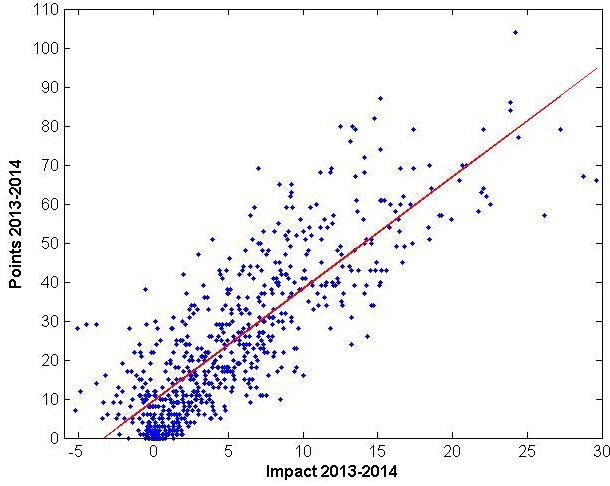
\includegraphics
[width = 0.6\columnwidth]
{points_vs_impact}
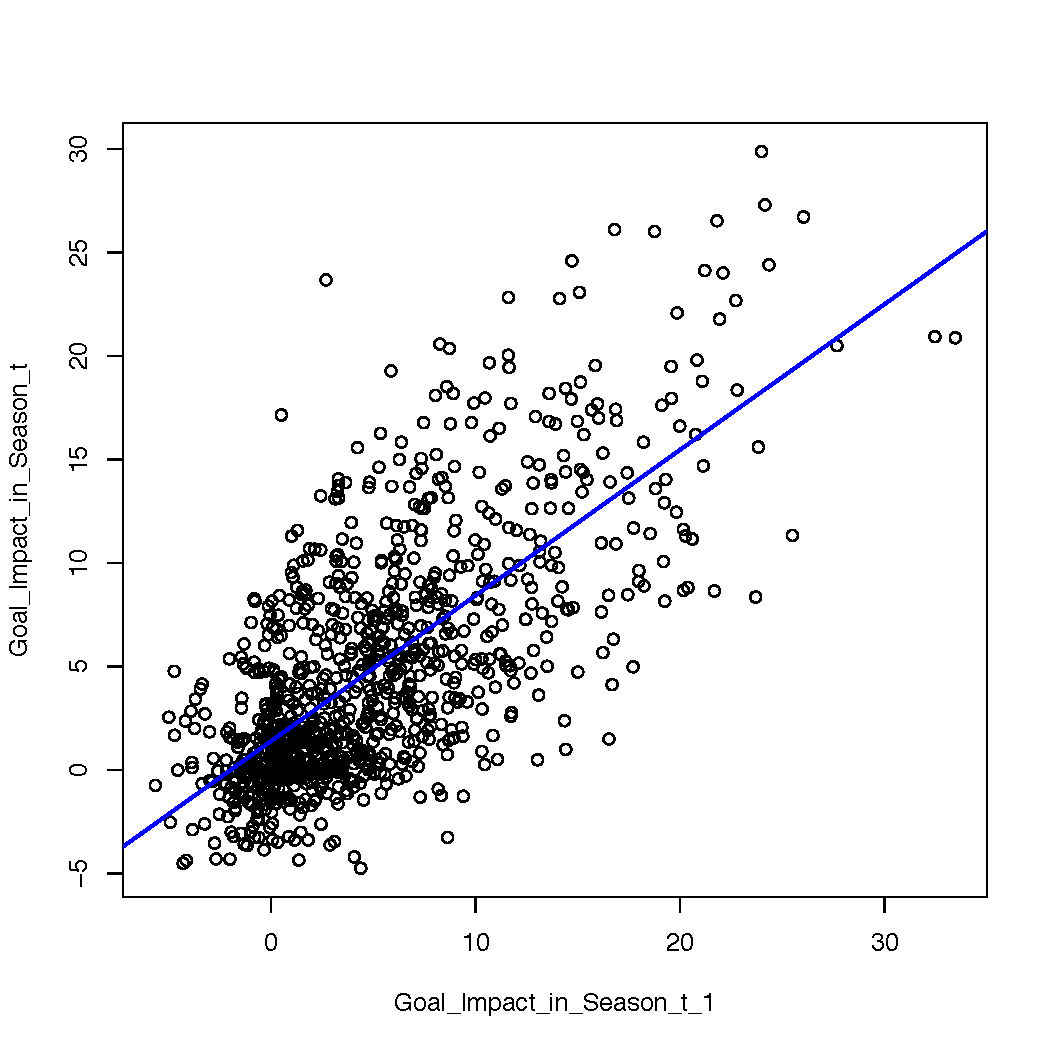
\includegraphics
[width = 0.6\columnwidth]
{correlation}
%\vspace{1in}
\caption{Left: 2013-2014 Correlation between Player Goal Impact and Points Earned. Right: Correlation between Goal Impact in one season and the next, for Seasons 2007-2014.}
\label{fig:points-vs-impact}
\end{figure}

\subsection{Case Studies} We discuss our findings for some individual players of interest.  Table~\ref{table:top-player-impact-goals} appears to pass the ``eye test'' in that it lists top offensive players of the NHL, including goal-getters such as Sidney Crosby, Steven Samkos, and Alex Ovechkin. The fact that these high scores are not ranked at the top illustrates the difference between goal impact and goals (cf.~\cite{Pettigrew2015}). All three members of St. Louis'  famed ``STL'' line
(Schwartz,  Tarasenko, Lehtera)\footnote{\url{http://www.nhl.com/ice/news.htm?id=738943}}   are among the top 20 in our list. In fact, Jori Lehtera tops our goal impact list, although his  linemate Tarasenko outscored him by far. Our analysis suggests that Lehtera's actions create the opportunities that Tarasenko exploits. This pattern fits the traditional division of labor between a center and a wing player. Tarasenko is also the most undervalued player in our list. Starting with the 2015-2016 season, St. Louis has signed him for an annual average of 7.5M contract, which our analysis strongly supports. 



Jason Spezza is an anomaly, as he has the third-highest impact score but a negative +/- score. This may be due to a lack of defensive contributions (defensive actions are underrepresented in the NHL data and therefore in the Q-value count). Another explanation is that while Spezza  generally performs useful actions, he happens to play on a relatively poor line. A strong example of this scenario was the 2013-2014 season, where Spezza topped our goal impact list, but had a very low +/- score of -26~\cite{Routley2015a}. This reason for this score is that his Ottawa team performed poorly overall in the 2013-2014 season, with a goal differential of -29. Spezza requested a trade, which our analysis would recommend. At the Dallas Stars, his season total +/- score was more in line with his goal impact as we would predict. (-7 compared to Dallas' +1 overall).

\section{Goal Impact Is Consistent Across Seasons.}

A desirable feature of a player ranking score is temporal consistency~\cite{Pettigrew2015}, for at least two reasons. First, generally the skill of a player does not change greatly from one season to the next. Therefore a good quality metric should show consistency between seasons. Second, a consistent ranking is useful because it supports predicting future performance in the next season from past performance in previous seasons. To assess consistency across seasons, we follow Pettigrew's methodology~\cite{Pettigrew2015}. (1) For each pair of successive seasons, for each player who plays in both seasons, list the player score in each season. (2) Compute the correlation between players' impact score in season $t$ and the score in season $t+1$.
%
%\begin{enumerate}
%\item For each pair of successive seasons, for each player who plays in both seasons, list the player score in each season.
%\item Compute the correlation between the impact score in season $t$ and the score in season $t+1$.
%\end{enumerate}
%
Table~\ref{table:correlation} shows the season-to-season correlation for the goal impact scores and related measures. {\em Goal impact as defined by the Markov game model is well correlated across seasons}, $r = 0.71$. The trend line in the scatter plot of Figure~\ref{fig:points-vs-impact} (right) shows the correlation graphically. In contrast, the traditional +/- score varies across seasons, $r = 0.345$. Table~\ref{table:correlation} also shows cross-season correlations for a number of adjusted goal impact (GI) metrics: goal season impact per total games played in season (similar to \cite{Pettigrew2015}), impact per minutes played, and impact per actions taken. All of the adjusted metrics are substantially less consistent than the summed goal impact metric.

An interesting computation for future work would be to focus the correlations on players who change teams. We would predict that Goal Impact remains consistent across seasons for such players, as it reflects their individual achievement, whereas goal-based scores like +/- and points depend heavily on a player's teammates and should therefore be less consistent when players change teams.\footnote{We are indebted to an anonymous workshop reviewer for this suggestion.}

\begin{table}[htb]
\caption{Season-to-Season Correlations for Different Player Performance Metrics.}
\label{table:correlation}
\begin{center}
\resizebox{0.6\columnwidth}{!}{
\begin{tabular}{|c|c|c|c|c|}
\hline
\bf{Goal Impact} & \bf{PlusMinus} & \bf{GI/Games} & \bf{GI/Actions} & \bf{GI/TimePlayed}
 \\
\bf{0.703} & 0.345 & 0.508 & 0.141 & 0.325 \\\hline
\end{tabular}
}
\end{center}
\end{table}

\section{Conclusion}
We have described a Markov Game Model for a massive set of NHL play-by-play events with a rich state space. % that utilizes much of the information in the data.
Compared to previous work that assigns a single value to actions, the model's action-value Q-function incorporates two powerful sources of information for valuing hockey actions: (1) It takes into account the context of the action, represented by the Markov Game state. (2) It models the medium-term impact of an action by propagating its effect to future states. %The Q-function provides knowledge about hockey dynamics by quantifying how much which action matters when.
%Propagating action effects across sequences utilizes the ordering of play sequences in a game, rather than treating sequences as an unordered independent set.
%
We applied our model to evaluate the performance of players in terms of their actions' total impact.
%Action impact scores are calculated for players with respect to different objective functions.
%Impact scores for the next goal correlate with points. 
We showed that players' goal impact values are consistent and hence predictable across seasons. %Another potential application for context-aware performance evaluation is in finding strengths and weaknesses of teams: We can use the Q-function to find situations in which a teams mix of actions provides a substantially different expected result from a generic team.
In sum, the Q-function is a powerful AI concept that captures much information about hockey dynamics as the game is played in the NHL. While player ranking is one important application for hockey analytics, we expect that the Q-function concept will facilitate many others.

		\bibliographystyle{abbrv}
		\bibliography{master}
	\end{document}
	
